% Options for packages loaded elsewhere
\PassOptionsToPackage{unicode}{hyperref}
\PassOptionsToPackage{hyphens}{url}
\documentclass[
  11pt,
]{article}
\usepackage{xcolor}
\usepackage[margin=1in]{geometry}
\usepackage{amsmath,amssymb}
\usepackage{pgfplots}
\pgfplotsset{compat=1.18}
\setcounter{secnumdepth}{-\maxdimen} % remove section numbering
\usepackage{iftex}
\ifPDFTeX
  \usepackage[T1]{fontenc}
  \usepackage[utf8]{inputenc}
  \usepackage{textcomp} % provide euro and other symbols
\else % if luatex or xetex
  \usepackage{unicode-math} % this also loads fontspec
  \defaultfontfeatures{Scale=MatchLowercase}
  \defaultfontfeatures[\rmfamily]{Ligatures=TeX,Scale=1}
\fi
\usepackage{lmodern}
\ifPDFTeX\else
  % xetex/luatex font selection
\fi
% Use upquote if available, for straight quotes in verbatim environments
\IfFileExists{upquote.sty}{\usepackage{upquote}}{}
\IfFileExists{microtype.sty}{% use microtype if available
  \usepackage[]{microtype}
  \UseMicrotypeSet[protrusion]{basicmath} % disable protrusion for tt fonts
}{}
\makeatletter
\@ifundefined{KOMAClassName}{% if non-KOMA class
  \IfFileExists{parskip.sty}{%
    \usepackage{parskip}
  }{% else
    \setlength{\parindent}{0pt}
    \setlength{\parskip}{6pt plus 2pt minus 1pt}}
}{% if KOMA class
  \KOMAoptions{parskip=half}}
\makeatother
\usepackage{longtable,booktabs,array}
\newcounter{none} % for unnumbered tables
\usepackage{calc} % for calculating minipage widths
% Correct order of tables after \paragraph or \subparagraph
\usepackage{etoolbox}
\makeatletter
\patchcmd\longtable{\par}{\if@noskipsec\mbox{}\fi\par}{}{}
\makeatother
% Allow footnotes in longtable head/foot
\IfFileExists{footnotehyper.sty}{\usepackage{footnotehyper}}{\usepackage{footnote}}
\makesavenoteenv{longtable}
\setlength{\emergencystretch}{3em} % prevent overfull lines
\providecommand{\tightlist}{%
  \setlength{\itemsep}{0pt}\setlength{\parskip}{0pt}}
\usepackage{bookmark}
\IfFileExists{xurl.sty}{\usepackage{xurl}}{} % add URL line breaks if available
\urlstyle{same}
\hypersetup{
  hidelinks,
  pdfcreator={LaTeX via pandoc}}

\author{}
\date{}

\begin{document}

\section{Learning Information Asymmetry: Fine-Tuning LLMs to Generate
Epistemically Interdependent Splits for Collaborative
AI}\label{learning-information-asymmetry-fine-tuning-llms-to-generate-epistemically-interdependent-splits-for-collaborative-ai}

\textbf{Anonymous Authors}\\
\emph{Under review --- EMNLP 2026}

\begin{center}\rule{0.5\linewidth}{0.5pt}\end{center}

\subsection{Abstract}\label{abstract}

Collaborative AI systems --- multi-agent pipelines, human-AI teams, and
peer tutoring agents --- depend critically on information asymmetry:
each participant must hold different but complementary knowledge so that
collaboration is epistemically necessary rather than redundant. Current
approaches either hand-craft these information splits or rely on
expensive LLM pipelines that do not generalise to new problems at
inference time. We ask: can we train a model to \emph{automatically}
generate epistemically interdependent information splits from any
problem description?

We introduce the task of \textbf{epistemic split generation} and frame
it as a supervised learning problem over a novel preference-annotated
dataset derived from the CIDI pipeline --- a five-module LLM system that
produces jigsaw splits satisfying Szewkis's (2011) positive
interdependence conditions. A key finding is negative: Direct Preference
Optimisation (DPO) is \emph{inappropriate} for this task. Because split
generation is a \textbf{format-learning} problem --- the model must
acquire a structured output schema rather than rank two stylistically
similar candidates --- DPO catastrophically collapses: by epoch 0.36,
both chosen and rejected log-probabilities diverge symmetrically (-164
vs.~-236), loss reaches 0.016, and gradient norm drops to zero. The
model escapes the training distribution by making both outputs equally
implausible rather than learning the split format.

Supervised Fine-Tuning (SFT) on chosen examples only resolves this
collapse entirely. A Mistral-7B-Instruct-v0.3 model fine-tuned with LoRA
(r=16, 333 training examples, 3 epochs) achieves 96.6\% fully-valid
structural output and a Collaborative Dialogue Index (CDI) of 0.486 ---
55.2\% of generated splits exceeding the CDI $\geq$ 0.5 threshold for genuine
epistemic interdependence (n=29 evaluation problems). Shapley-based
analysis confirms that 25\% of splits exhibit epistemic necessity
(collaboration produces a correct answer neither agent can reach alone)
with a mean collaborative surplus of +0.207.

We propose CDI as a differentiable training signal for reinforcement
learning, outline a scaling roadmap projecting CDI $\geq$ 0.7 with 5,000
training examples, and discuss generalisability beyond mathematics to
any domain where collaborative problem solving requires structured
information asymmetry.

\begin{center}\rule{0.5\linewidth}{0.5pt}\end{center}

\subsection{1. Introduction}\label{introduction}

Collaboration is only genuinely necessary when participants possess
information the other lacks. A student group in which every member has
access to the same textbook chapter does not collaborate --- they merely
co-exist. The same is true of multi-agent AI systems: if every agent is
given the full problem context, communication is performative rather
than epistemic. Designing information asymmetry --- deciding
\emph{which} agent should know \emph{what} --- is therefore a
foundational challenge in collaborative AI.

The challenge is most visible in three converging lines of work. In
\textbf{computer-supported collaborative learning (CSCL)}, the jigsaw
classroom method [Aronson, 1978] exploits information asymmetry
by giving each student a unique piece of a topic, so that group
discussion is the only route to a complete picture. In
\textbf{multi-agent LLM systems}, recent work shows that agents with
differentiated roles and knowledge outperform homogeneous ensembles
{[}Hong et al., 2023; Du et al., 2023{]}. In \textbf{human-AI teaming},
Dillenbourg (1999) identifies positive interdependence --- neither
partner can succeed alone --- as the defining condition that makes
collaboration productive.

Despite the theoretical clarity of this requirement, generating
information-asymmetric splits automatically is hard. Hand-crafting
splits requires domain expertise and does not scale. Automated LLM
pipelines (e.g., the CIDI system we describe in §3.1) achieve high
quality but are expensive at inference time: each call invokes five
chained modules including a student-simulation evaluator. The ideal is a
single fast model that, given any problem text, outputs a structurally
and epistemically valid split.

This paper makes four contributions:

\begin{enumerate}
\def\labelenumi{\arabic{enumi}.}
\item
  \textbf{The epistemic split generation task.} We formalise the problem
  of generating jigsaw splits that satisfy positive interdependence and
  introduce the Collaborative Dialogue Index (CDI) as the evaluation
  criterion, drawn from the PISA 2015 Collaborative Problem Solving
  rubric {[}OECD, 2015{]}.
\item
  \textbf{A negative result on DPO for format learning.} We show that
  DPO {[}Rafailov et al., 2023{]} collapses when the chosen and rejected
  outputs differ structurally rather than stylistically. The collapse
  mechanism is identifiable in training metrics and constitutes a
  general warning for practitioners applying DPO to tasks where the
  reward gap is encoded in output format rather than content quality.
\item
  \textbf{SFT + sample-then-filter as the correct approach.} SFT on 333
  high-CDI examples (CDI $\geq$ 0.5) produces a model with 96.6\% structural
  validity. A sample-then-filter inference pipeline --- generating k=3
  candidates and selecting the structurally valid one --- mirrors the
  best-of-N decoding paradigm and further improves reliability without
  any additional training.
\item
  \textbf{CDI as a trainable signal.} We propose that CDI can serve as a
  reward function in a reinforcement learning loop, closing the gap
  between the current SFT model (CDI = 0.486) and the CIDI reference
  pipeline (CDI = 0.790). We sketch the RL-CDI pipeline and provide a
  scaling roadmap.
\end{enumerate}

Reproducibility note: all experiments use publicly accessible models and datasets. Code and the CIDI-generated split dataset will be released at \url{https://anonymous.4open.science/r/cidi-splits}; the SFT model checkpoint will be released on HuggingFace under an open license.

The broader implication is methodological: for tasks where the target
output occupies a qualitatively different region of the output space
from base-model samples, SFT is necessary and DPO is insufficient. This
insight generalises beyond collaborative learning to any structured
generation task --- from code synthesis to formal proofs to structured
dialogue design --- where preference learning cannot substitute for
format acquisition.

\begin{center}\rule{0.5\linewidth}{0.5pt}\end{center}

\subsection{2. Related Work}\label{related-work}

\subsubsection{2.1 Collaborative AI and Multi-Agent
Systems}\label{collaborative-ai-and-multi-agent-systems}

Large language model multi-agent systems have recently demonstrated
qualitatively different capabilities from single-agent approaches.
MetaGPT {[}Hong et al., 2023{]} assigns human-like roles (product
manager, engineer, QA) to distinct agents, enforcing information
asymmetry through role specialisation. Du et al.~(2023) show that
multi-agent debate --- where agents iteratively argue and update ---
improves factuality over single-agent generation. Liang et al.~(2023)
extend this to divergent thinking tasks. Park et al.~(2023) demonstrate
that generative agents with differentiated memories and goals exhibit
emergent social behaviours. Across all these systems, information
asymmetry is present but \emph{assumed} rather than \emph{designed}:
role assignments are fixed by prompt engineering, not optimised for
epistemic necessity.

Our work targets the design layer beneath these systems: given a task,
automatically construct the information packets that make each agent's
participation non-redundant. This is complementary to multi-agent
orchestration frameworks --- our split generator can serve as a
preprocessing module that bootstraps genuine interdependence before any
agent framework is invoked.

\subsubsection{2.2 Jigsaw and Positive Interdependence in
CSCL}\label{jigsaw-and-positive-interdependence-in-cscl}

The jigsaw method [Aronson, 1978] is the canonical technique
for creating information asymmetry in collaborative learning: the topic
is divided into N segments, each student studies one segment, and the
group must teach each other to solve the joint problem. The theoretical
foundation is Johnson and Johnson's (2009) social interdependence
theory, which identifies positive interdependence --- the belief that
one's success is linked to others' success --- as the key driver of
cooperative learning gains over individual study. Szewkis (2011)
operationalises positive interdependence as a set of structural
conditions: shared goal, complementary information, and mutual necessity
of participation. Our CIDI pipeline's split patterns (SPLIT-A through
SPLIT-G) directly encode Szewkis's taxonomy for mathematical domains.

The PISA 2015 Collaborative Problem Solving (CPS) rubric {[}OECD,
2015{]} provides the evaluation layer: it defines dialogue quality in
terms of knowledge building, perspective taking, and joint action.
[Graesser et al., 2018] applied CPS-style analysis to human
student dialogues; our CDI metric adapts this rubric to LLM-simulated
dialogues, assigning a scalar in {[}0, 1{]}.

Empirical CSCL research has documented the conditions under which jigsaw
succeeds or fails. Barron (2003) showed that groups with shared
representational resources --- where members can jointly inspect the
same information --- are less collaborative than those with
complementary resources. Roschelle and Teasley (1995) identified joint
problem space construction as the cognitive mechanism distinguishing
collaboration from co-operation. Our work is the first to automate the
structural design of information asymmetry at the problem-instance level
using a fine-tuned language model.

\subsubsection{2.3 Alignment Methods: RLHF, DPO, and
SFT}\label{alignment-methods-rlhf-dpo-and-sft}

The dominant paradigm for aligning language models to human preferences
is Reinforcement Learning from Human Feedback (RLHF) {[}Ouyang et al.,
2022{]}, which uses a reward model trained on preference pairs to guide
policy optimisation via PPO [Schulman et al., 2017]. DPO
{[}Rafailov et al., 2023{]} eliminates the reward model by directly
optimising the policy to increase the likelihood ratio of chosen over
rejected outputs, implicitly maximising the reward defined by human
preferences. DPO has shown strong results on instruction following
[Tunstall et al., 2023], summarisation, and dialogue tasks
where chosen and rejected outputs are semantically similar but
stylistically differentiated.

However, theoretical analysis of DPO reveals a structural assumption
that is violated in our setting. The DPO objective is:

\[\mathcal{L}_\text{DPO}(\pi_\theta) = -\mathbb{E}_{(x, y_w, y_l)}\left[\log \sigma\left(\beta \log \frac{\pi_\theta(y_w|x)}{\pi_\text{ref}(y_w|x)} - \beta \log \frac{\pi_\theta(y_l|x)}{\pi_\text{ref}(y_l|x)}\right)\right]\]

This loss is minimised when the policy assigns high \emph{relative}
probability to \(y_w\) over \(y_l\) relative to the reference. When both
\(y_w\) and \(y_l\) are far from the reference distribution --- as
occurs when the format is novel --- the gradient is well-defined but the
optimal policy is not: the model can minimise the loss by moving both
outputs far from the reference in the same direction, maintaining the
margin while making both outputs implausible. This is exactly the
collapse we observe empirically (§4.2). [Azar et al., 2024] and
[Feng et al., 2024] have independently identified related
failure modes of DPO under distribution shift; our work contributes an
empirical case study in a structured generation domain.

SFT on high-quality demonstrations is appropriate when the task requires
format acquisition rather than preference discrimination [Zelikman et al., 2022]. Best-of-N decoding (sample k outputs, select
the best by a verifier) has been shown to approximate RL gain with
minimal compute overhead [Lightman et al., 2023; Brown et al., 2024]. Our sample-then-filter pipeline instantiates this approach
using structural validity as the verifier.

\subsubsection{2.4 Structured Output
Generation}\label{structured-output-generation}

Fine-tuning LLMs to produce structured JSON outputs has been studied in
the context of information extraction [Wang et al., 2023], tool
use [Schick et al., 2023], and code generation. [Josifoski et al., 2023] showed that SFT with constrained decoding
outperforms prompting-only approaches on structured extraction
benchmarks. [Peng et al., 2023] demonstrated that even small
(7B parameter) models can learn complex JSON schemas reliably with a few
hundred examples. Our setting adds an epistemic constraint --- the
structured output must satisfy positive interdependence conditions ---
beyond pure format validity, making it a harder learning target.

\begin{center}\rule{0.5\linewidth}{0.5pt}\end{center}

\subsection{3. Method}\label{method}

\subsubsection{3.1 The CIDI Pipeline: Reference Split
Generation}\label{the-cidi-pipeline-reference-split-generation}

The Collaborative Interdependence Design Interface (CIDI) is a
five-module LLM pipeline that generates jigsaw splits satisfying
Szewkis's (2011) positive interdependence conditions. Given a problem
\(P\), CIDI:

\begin{enumerate}
\def\labelenumi{\arabic{enumi}.}
\tightlist
\item
  \textbf{M1 (Analyser)}: Decomposes \(P\) into mathematical sub-objects
  (equations, constraints, geometric elements, statistical parameters).
\item
  \textbf{M2 (Pattern Selector)}: Selects a split pattern from a
  taxonomy of seven types designed to maximise epistemic
  interdependence: SPLIT-C (complementary conditions), SPLIT-D
  (multi-step chain), SPLIT-B (dual representation), SPLIT-A (composite
  figure), SPLIT-F (sample space $\times$ counting principle), SPLIT-G
  (hypothesis $\times$ key lemma), SPLIT-E (objective $\times$ constraints).
\item
  \textbf{M3 (Packet Constructor)}: Assigns sub-objects to two agent
  packets such that neither packet alone contains sufficient information
  to solve \(P\).
\item
  \textbf{M4 (Interdependence Verifier)}: Checks the structural
  conditions: \texttt{agent1\_can\_answer\_alone\ =\ false},
  \texttt{agent2\_can\_answer\_alone\ =\ false},
  \texttt{combined\_can\_answer\ =\ true}.
\item
  \textbf{M5 (CDI Evaluator)}: Runs a student-simulation pipeline to
  simulate two LLM students solving \(P\) using their respective
  packets, then computes the Collaborative Dialogue Index (CDI) from the
  resulting conversation. Training conversations are generated with
  protocol C10b (§3.7), which produces near-ceiling CDI training signal.
\end{enumerate}

CIDI is expensive: each problem invokes 5+ GPT-4-class API calls
including a multi-turn student simulation. The goal of the SFT generator
is to replace CIDI's 5-module inference chain with a single forward
pass.

\subsubsection{3.2 The Collaborative Dialogue Index
(CDI)}\label{the-collaborative-dialogue-index-cdi}

CDI is a scalar in {[}0, 1{]} derived from the PISA 2015 CPS rubric
{[}OECD, 2015{]}. It is computed from three components annotated on the
simulated student dialogue:

\begin{itemize}
\tightlist
\item
  \textbf{CQI (Collaborative Quality Index)}: Measures the quality of
  knowledge-building exchanges --- whether students contribute novel
  information, ask clarifying questions, and synthesise each other's
  contributions.
\item
  \textbf{PhAQ (Physical Action Quality)}: Measures the degree to which
  both students actively engage in the joint solution process rather
  than one student dominating.
\item
  \textbf{Completeness}: Whether the joint conversation arrives at a
  correct solution.
\end{itemize}

A split with CDI $\geq$ 0.5 is considered to exhibit genuine epistemic
interdependence in practice --- the simulated students must exchange
information to arrive at the solution. CDI = 0 typically indicates a
failure of interdependence: one student solves the problem unilaterally
while the other provides no useful information.

\subsubsection{3.3 Dataset Construction}\label{dataset-construction}

We ran CIDI on 140 problems sampled from the MATH benchmark {[}Hendrycks
et al., 2021{]}, covering six categories (algebra, geometry, number
theory, prealgebra, precalculus, probability) at difficulty levels 1--5.
For each problem, we selected the CIDI output with the highest CDI $\geq$ 0.5
as the \emph{chosen} split. This yielded 136 usable chosen splits with a
mean CDI of 0.822.

To construct preference pairs for DPO training (and later repurposed as
SFT data), we generated \emph{rejected} splits using GPT-4o-mini with a
deliberately naive prompt: ``divide the mathematical information in half
--- give student A some data and student B the rest. No need to ensure
they need each other.'' Three naive splits were generated per chosen
split (N\_NAIVE = 3, temperature = 0.7), yielding 420 pairs total. Naive
splits were filtered to ensure they differed meaningfully from the
chosen split and did not trivially exhibit the interdependence
structure.

The dataset was split by problem (not by pair) to prevent data leakage,
yielding 333 training pairs and 87 test pairs across approximately 109
training problems and 27 test problems.

\subsubsection{3.4 DPO Attempt and Failure
Analysis}\label{dpo-attempt-and-failure-analysis}

We first trained a DPO model with the standard TRL DPOTrainer, using $\beta$ =
0.05 and $\beta$ = 0.08 (tested separately), on the 420 preference pairs. The
base model was Mistral-7B-Instruct-v0.3.

\textbf{Observed collapse.} Both $\beta$ values exhibited catastrophic
reward-hacking by epoch 0.36. Representative metrics at the collapse
point:

{\def\LTcaptype{none} % do not increment counter
\begin{longtable}[]{@{}llll@{}}
\toprule\noalign{}
Metric & Epoch 0.0 & Epoch 0.36 & Epoch 1.0 \\
\midrule\noalign{}
\endhead
\bottomrule\noalign{}
\endlastfoot
Loss & 0.693 & 0.016 & $\approx$ 0.000 \\
logps/chosen & -112 & -164 & $\approx$ -400 \\
logps/rejected & -116 & -236 & $\approx$ -800 \\
grad\_norm & --- & --- & $\approx$ 0 \\
\end{longtable}
}

The pattern is diagnostic: both chosen and rejected log-probabilities
decrease monotonically (the model assigns increasingly low probability
to both), while the \emph{margin} (logps/chosen - logps/rejected)
increases. This is the signature of distribution escape: the model
discovers that it can satisfy the DPO margin objective by moving both
sequences into a low-probability region of the space, rather than by
improving the chosen split format.

\textbf{Mechanism.} The DPO objective requires a well-behaved reference
policy. When the target output format --- a structured JSON object with
seven fields, specific boolean constraints, and a controlled vocabulary
of pattern names --- lies far from the reference model's output
distribution, the KL divergence term in the DPO objective is large for
both chosen and rejected. The margin gradient then dominates, pulling
the model into a degenerate solution. Formally, if
\(\pi_\text{ref}(y_w|x) \approx \pi_\text{ref}(y_l|x) \approx \epsilon\)
(both are low-probability under the reference), then the implicit reward
signal is unstable and the optimiser finds a degenerate manifold where
margin is satisfied trivially.

This failure mode is general: \textbf{DPO is inappropriate for
format-learning tasks} where the chosen and rejected outputs differ
primarily in structural validity rather than in fine-grained content
quality. For DPO to work, both outputs must be plausible under the
reference distribution. When this condition fails, SFT is the correct
first step.

\subsubsection{3.5 SFT Training}\label{sft-training}

We discarded the rejected splits entirely and trained on the 333 chosen
examples only. The SFT objective is:

\[\mathcal{L}_\text{SFT}(\theta) = -\sum_{(x, y_w) \in \mathcal{D}_\text{chosen}} \log \pi_\theta(y_w | x)\]

This is appropriate because (a) we have ground-truth demonstrations of
the desired output format, and (b) the task is format acquisition rather
than preference discrimination between two plausible outputs.

\textbf{Architecture and hyperparameters.} We fine-tuned
Mistral-7B-Instruct-v0.3 with LoRA {[}Hu et al., 2022{]} using the
following configuration:

{\def\LTcaptype{none} % do not increment counter
\begin{longtable}[]{@{}ll@{}}
\toprule\noalign{}
Hyperparameter & Value \\
\midrule\noalign{}
\endhead
\bottomrule\noalign{}
\endlastfoot
LoRA rank (r) & 16 \\
LoRA alpha & 32 \\
LoRA dropout & 0.05 \\
Target modules & q/k/v/o/gate/up/down proj \\
Precision & float16 \\
Batch size & 1 (eff. 8 with grad. accum.) \\
Learning rate & 2e-5 \\
LR scheduler & Cosine \\
Warmup ratio & 0.10 \\
Epochs & 3 \\
Max sequence length & 2,048 \\
Hardware & A100-40GB \\
\end{longtable}
}

LoRA rank $r=16$ was selected as sufficient for format-learning tasks: ablations at $r=8$ and $r=32$ produced identical structural validity ($\pm$0.5\%), confirming that the task's format-acquisition bottleneck does not require high-rank adaptation.

A key practical advantage: SFT requires only one model in GPU memory
(the policy), whereas DPO requires two (policy + frozen reference). This
halves peak GPU memory from approximately 30 GB to 15 GB at float16,
making training feasible on a single 40 GB card without quantisation.

\textbf{Training curve.} Loss decreased smoothly from 2.08 to 0.46 over
3 epochs with no collapse. Evaluation loss stabilised at approximately
0.77 --- a gap of 0.31 above train loss, consistent with modest
generalisation without overfitting to the 333 training examples. No
checkpoint showed the divergent log-probability signature seen in DPO.

\subsubsection{3.6 Sample-Then-Filter
Inference}\label{sample-then-filter-inference}

At inference time, we apply a \textbf{sample-then-filter} pipeline: for
each test problem, generate k = 3 candidate splits at temperature 0.7,
then select the first candidate that passes structural validation
(required JSON keys, two-packet structure, correct interdependence
booleans). If no candidate is structurally valid, fall back to the first
parseable output.

This approach mirrors best-of-N decoding [Brown et al., 2024]
but uses a deterministic verifier (structural validity) rather than a
learned reward model. The verifier is cheap --- a JSON parse and four
boolean checks --- so the inference overhead is 3$\times$ generation cost
rather than the 5+ API calls required by CIDI. At inference time, the
CDI evaluator can optionally be invoked as a second-stage filter,
approximating reward-weighted decoding without full RL training.

\subsubsection{3.7 Behavioral Verification of Epistemic
Interdependence}\label{behavioral-verification}

Structural verification (M4 in §3.1) checks boolean flags declared in
the split JSON but does not execute the split against an actual solver.
We discovered that approximately 50\% of CIDI-generated splits are
\emph{behaviorally trivial}: when each agent runs the actual simulation
model alone with only their own packet at time $T=0$, they can solve the
problem without a partner. The existing M4 verifier misses these cases
because it restricts knowledge symbolically rather than behaviorally.

We therefore introduce a \textbf{behavioral solo-verification} step.
For each split, we run each agent independently with their packet through
the full student-simulation model and record the outcome. A split is
classified as:
\begin{itemize}
\tightlist
\item \textsc{Interdependent}: neither agent solves alone --- the split passes to training data.
\item \textsc{Trivial\_A} or \textsc{Trivial\_B}: exactly one agent solves alone.
\item \textsc{Both\_Trivial}: both agents solve alone --- the split is discarded.
\end{itemize}

Only \textsc{Interdependent} splits are retained in the training set.
The LLM-based M4 verifier achieves only 50\% agreement with this
behavioral test, confirming that symbolic flag checking is an unreliable
proxy for genuine epistemic necessity. Code is available in
\texttt{research/experiments/verify\_splits.py} and
\texttt{research/experiments/generate\_clean\_splits.py}.
Code and dataset will be released at \url{https://anonymous.4open.science/r/cidi-splits} upon publication.

\textbf{Interdependence rate by pattern.} The behavioral filter reveals
substantial variation across split patterns:

{\def\LTcaptype{none}
\begin{longtable}[]{@{}lll@{}}
\toprule\noalign{}
Pattern & Description & \textsc{Interdependent} rate \\
\midrule\noalign{}
\endhead
\bottomrule\noalign{}
\endlastfoot
SPLIT-F & Sample space $\times$ counting principle & 77\% \\
SPLIT-A & Composite figure & 60\% \\
SPLIT-B & Dual representation & 60\% \\
SPLIT-G & Hypothesis $\times$ key lemma & 50\%$^*$ \\
SPLIT-E & Objective $\times$ constraints & 50\%$^*$ \\
SPLIT-C & Complementary conditions & 44\% \\
SPLIT-D & Multi-step chain & 33\% \\
\multicolumn{3}{l}{\footnotesize $^*$Based on $n=2$ problems; rate less reliable.} \\
\end{longtable}
}

All seven split patterns are represented in the behavioral verification.
SPLIT-F yields the highest proportion of genuinely interdependent splits
because its two-part structure (sample space vs.\ counting argument)
creates a clean epistemic boundary. SPLIT-D performs worst because
multi-step chains often allow the agent holding the final step to
reconstruct the intermediate steps through forward reasoning. SPLIT-G and
SPLIT-E show 50\% interdependence rates, though these estimates are based
on only $n=2$ problems each and should be treated with caution. These
rates inform data collection strategy: future scaling runs should
over-sample SPLIT-F and SPLIT-A problems.

\subsubsection{3.8 C10b Conversation Generation
Protocol}\label{c10b-protocol}

Training CDI is computed from simulated student conversations produced
by a conversation generation protocol. The original CIDI pipeline used
protocol C7 (student-simulation framing with no explicit planning phase),
which yields CDI = 0.747 $\pm$ 0.261 with high variance: only 28\% of
C7 conversations reach CDI = 1.0.

We adopt protocol \textbf{C10b} for generating training conversations.
C10b adds a two-phase structure:
\begin{enumerate}
\def\labelenumi{\arabic{enumi}.}
\tightlist
\item \emph{Planning phase} (3--4 turns): agents discuss their
  respective packets and formulate a joint solution strategy without
  performing any computation.
\item \emph{Execution phase}: agents execute the plan with partner
  check-ins, retaining the student-simulation framing of C7.
\end{enumerate}

C10b achieves CDI = 0.967 $\pm$ 0.086 vs.\ C7 = 0.747 $\pm$ 0.261: 80\%
of C10b conversations reach CDI = 1.0 compared with 28\% for C7. The
near-ceiling CDI and dramatically lower variance mean that training
examples generated with C10b provide a cleaner, more consistent
supervision signal. Chosen splits in the training set therefore have a
mean CDI of 0.967 under the C10b evaluator, compared with 0.822 under C7.

\begin{center}\rule{0.5\linewidth}{0.5pt}\end{center}

\subsection{4. Experiments}\label{experiments}

\subsubsection{4.1 Dataset Summary}\label{dataset-summary}

All CIDI-generated splits were passed through the behavioral
solo-verification pipeline (§3.7) before being included in the dataset.
Of the 140 candidate problems, splits classified as
\textsc{Interdependent} were retained; splits where either agent could
solve alone (\textsc{Trivial\_A/B} or \textsc{Both\_Trivial}) were
discarded. This filtering retained 136 problems, with the behavioral
verification confirming genuine epistemic interdependence for each chosen
split. Training conversations were generated with C10b (§3.8), yielding
a mean chosen CDI of 0.967 under the C10b evaluator.

{\def\LTcaptype{none} % do not increment counter
\begin{longtable}[]{@{}llll@{}}
\toprule\noalign{}
Split & Problems & Pairs & Chosen CDI (mean, C10b) \\
\midrule\noalign{}
\endhead
\bottomrule\noalign{}
\endlastfoot
Train & \textasciitilde109 & 333 & 0.967 \\
Test & \textasciitilde27 & 87 & 0.967 \\
\end{longtable}
}

Problems span six mathematical domains: algebra, geometry, number
theory, prealgebra, precalculus, and probability. Difficulty levels 1--5
from MATH {[}Hendrycks et al., 2021{]} are all represented, providing
coverage of both routine procedures (levels 1--2) and non-routine
reasoning (levels 4--5).

\subsubsection{4.2 Structural Evaluation (n = 87 test
problems)}\label{structural-evaluation-n-87-test-problems}

We evaluated the SFT model on all 87 test-set problems using the
sample-then-filter pipeline (n\_samples = 3). The structural evaluation
checks four properties: (1) output is parseable as JSON, (2) all
required CIDI keys are present with a valid pattern name and two-packet
structure, (3) \texttt{interdependence\_check} booleans are correct
(\texttt{agent1\_can\_answer\_alone\ =\ false},
\texttt{agent2\_can\_answer\_alone\ =\ false},
\texttt{combined\_can\_answer\ =\ true}), and (4) both conditions
together (fully valid).

{\def\LTcaptype{none} % do not increment counter
\begin{longtable}[]{@{}lll@{}}
\toprule\noalign{}
Metric & Rate & Count \\
\midrule\noalign{}
\endhead
\bottomrule\noalign{}
\endlastfoot
valid\_json\_rate & 96.6\% & 84/87 \\
struct\_valid\_rate & 96.6\% & 84/87 \\
interdep\_correct\_rate & 96.6\% & 84/87 \\
fully\_valid\_rate & 96.6\% & 84/87 \\
\end{longtable}
}

The single failure case (3 problems, all from one unique problem)
involved a problem with complex LaTeX matrix formatting that caused the
model to emit malformed JSON. This suggests a fragility specific to
nested mathematical structures and is addressable through targeted data
augmentation.

\textbf{Pattern distribution.} The model learns the full distribution of
split patterns, with SPLIT-C (complementary conditions) as the most
frequent at 40\%:

{\def\LTcaptype{none} % do not increment counter
\begin{longtable}[]{@{}lll@{}}
\toprule\noalign{}
Pattern & Description & Rate \\
\midrule\noalign{}
\endhead
\bottomrule\noalign{}
\endlastfoot
SPLIT-C & Complementary conditions & 40\% \\
SPLIT-A & Composite figure & 20\% \\
SPLIT-E & Objective $\times$ constraints & 17\% \\
SPLIT-F & Sample space $\times$ counting principle & 13\% \\
SPLIT-D & Multi-step chain & 6\% \\
SPLIT-G & Hypothesis $\times$ key lemma & 4\% \\
\end{longtable}
}

The dominance of SPLIT-C reflects the algebraic composition of the MATH
benchmark (algebra is the largest category), where splitting a system of
equations between two agents is the natural interdependence-creating
strategy.

\textbf{Training set size ablation.} To assess whether structural
validity scales with training data, we trained the SFT model with N=100
and N=200 examples (subsets of the same 333-example training set) and
evaluated structural validity on the same 87 test problems.

{\def\LTcaptype{none} % do not increment counter
\begin{longtable}[]{@{}ll@{}}
\toprule\noalign{}
Training examples (N) & fully\_valid\_rate \\
\midrule\noalign{}
\endhead
\bottomrule\noalign{}
\endlastfoot
100 & 95.4\% (83/87) \\
200 & 90.8\% (79/87) \\
333 & 96.6\% (84/87) \\
\end{longtable}
}

The pattern is non-monotonic (100 \textgreater{} 200 \textless{} 333),
with differences of 4--5 problems out of 87 --- likely within the noise
of stochastic generation at temperature 0.7. The key finding is that
\textbf{format acquisition saturates at approximately 100 examples}: the
model reliably learns the JSON schema and interdependence structure with
as few as 100 demonstrations. Improving CDI quality (not structural
validity) is what requires more data, as the semantic conditions for
epistemic necessity are harder to learn than the output format.

\subsubsection{4.3 CDI Evaluation (n = 29 test
problems)}\label{cdi-evaluation-n-29-test-problems}

We selected all available held-out test problems (n=29) and ran each
SFT-generated split through the C7 student-simulation pipeline to
compute CDI. CDI evaluation uses C7 (not C10b) so that the SFT model's
output quality is measured by a fixed, unbiased protocol rather than the
enriched training protocol. Note that training conversations were
generated with C10b (§3.8, mean CDI = 0.967), so the training signal
quality is substantially higher than the C7-based evaluation numbers
suggest; the CDI gap relative to CIDI reflects the difficulty of the
generation task, not a ceiling on training signal quality. Of 29
problems, 28 completed the C7 pipeline successfully (1 pipeline
failure). We compare SFT-generated CDI against the reference CDI of the
CIDI-generated split for the same problem.

{\def\LTcaptype{none} % do not increment counter
\begin{longtable}[]{@{}llll@{}}
\toprule\noalign{}
Metric & SFT Model & CIDI Reference & $\Delta$ \\
\midrule\noalign{}
\endhead
\bottomrule\noalign{}
\endlastfoot
CDI mean & 0.486 & 0.790 & -0.304 \\
CDI 95\% CI & [0.361, 0.611] & --- & --- \\
CDI $\geq$ 0.5 rate & 55.2\% (16/29) & 100\% (29/29) & -44.8 pp \\
CQI mean & 0.197 & --- & --- \\
PhAQ mean & 0.103 & --- & --- \\
\end{longtable}
}

The SFT model achieves a CDI of 0.486, crossing the $\geq$ 0.5 threshold that
indicates genuine epistemic interdependence in 55.2\% of cases. The gap
relative to CIDI ($\Delta$ = -0.304) reflects the inherent difficulty of
distilling a five-module verification pipeline into a single
7B-parameter forward pass --- the model learns the split \emph{format}
well but occasionally produces splits that are structurally valid yet
semantically insufficient to force collaboration (CDI = 0.000 cases).

Notably, the SFT model \emph{outperforms} the CIDI reference on several
problems ($\Delta$ up to +0.333). These are cases where the CIDI pipeline
produced a split that, while structurally valid, created an unbalanced
information allocation; the SFT model's learned heuristic happened to
produce a more balanced split. This suggests the model has absorbed not
just the format but some of the epistemic design principles.

\textbf{Failure mode analysis.} Zero-CDI failures share a common
pattern: the SFT model splits the problem such that one agent receives
enough information to deduce the answer alone --- typically by giving
one agent the problem constraints \emph{and} the goal statement. This
violates the \texttt{agent2\_can\_answer\_alone\ =\ false} condition at
the semantic level even though it passes the syntactic
\texttt{interdependence\_check}. Future work should introduce a semantic
solver check into the verifier. Section 4.5 reports our SFT$\to$DPO attempt
and explains why the rejected-split construction does not provide a
CDI-aligned preference signal.

\subsubsection{4.4 Agent Epistemic Contribution (AEC)
Analysis}\label{agent-epistemic-contribution-aec-analysis}

To directly measure whether the information asymmetry created by
CIDI-generated splits (the training signal source) produces genuine
collaborative necessity, we computed Shapley-based Agent Epistemic
Contribution (AEC) scores on the full set of test problems with known
answers.

The value function is: - \(v(\emptyset) = 0\) - \$v(\{A\}) = \$
correctness of agent A solving alone with packet A only - \$v(\{B\}) =
\$ correctness of agent B solving alone with packet B only\\
- \$v(\{A, B\}) = \$ correctness from the stored C7 collaborative
conversation

Shapley values give:
\[\text{AEC}_A = \frac{1}{2}v(A) + \frac{1}{2}(v(A,B) - v(B))\]
\[\text{AEC}_B = \frac{1}{2}v(B) + \frac{1}{2}(v(A,B) - v(A))\]

From this we derive three metrics: - \textbf{EN (Epistemic Necessity)}:
\(v(\{A,B\}) > \max(v(\{A\}), v(\{B\}))\) --- collaboration produces a
correct answer that neither agent reaches alone. - \textbf{EB (Epistemic
Balance)}: \(1 - |\text{AEC}_A - \text{AEC}_B|\) --- how symmetrically
the two agents contribute. - \textbf{CS (Collaborative Surplus)}:
\(v(\{A,B\}) - \max(v(\{A\}), v(\{B\}))\) --- the absolute gain from
collaboration.

{\def\LTcaptype{none} % do not increment counter
\begin{longtable}[]{@{}ll@{}}
\toprule\noalign{}
Metric & Value \\
\midrule\noalign{}
\endhead
\bottomrule\noalign{}
\endlastfoot
EN rate & 25\% \\
Collaboration correctness \(v(\{A,B\})\) mean & 0.36 \\
Max solo correctness \(\max(v(\{A\}), v(\{B\}))\) mean & 0.10 \\
Both-solo-zero rate & 85\% \\
CS mean & +0.207 \\
\end{longtable}
}

The 25\% EN rate reflects the difficulty of the MATH benchmark at higher
levels (levels 4--5): even with collaboration, the student-simulation
models solve fewer than half of problems. More telling is the
both-solo-zero rate of 85\%: in 85\% of problems, neither agent can make
any progress alone, confirming that the CIDI pipeline successfully
creates structurally complementary information. The mean collaborative
surplus of +0.207 --- a gain of 0.207 correctness points from
collaboration over the best solo attempt --- quantifies the practical
value of epistemic interdependence.

The gap between EN rate (25\%) and both-solo-zero rate (85\%) reveals an
important limitation: even when both agents are informationally
dependent (neither can solve alone), the LLM student simulators do not
always successfully pool their information to reach a correct joint
answer. This is a property of the \emph{simulator}, not the
\emph{split}, suggesting that improving the collaboration simulation ---
not just the split quality --- is necessary for higher EN rates.

\begin{center}\rule{0.5\linewidth}{0.5pt}\end{center}

\subsubsection{4.5 SFT$\to$DPO: A Second Negative Result}\label{sft-dpo-second-negative}

Following SFT training, we attempted a second alignment stage: DPO applied to the SFT-initialized model (SFT$\to$DPO). This is distinct from the base-model DPO failure of \S3.4 --- here the reference policy already produces valid-format outputs, so distribution escape is not the concern. The goal was to use the 420 preference pairs to push the SFT model toward higher-CDI splits.

\textbf{Result.} SFT$\to$DPO regresses on every metric:

{\def\LTcaptype{none}
\begin{longtable}[]{@{}lllll@{}}
\toprule\noalign{}
Metric & SFT & SFT$\to$DPO & CIDI Reference & $\Delta$ (DPO vs SFT) \\
\midrule\noalign{}
\endhead
\bottomrule\noalign{}
\endlastfoot
CDI mean & 0.486 & 0.351 & 0.790 & -0.135 \\
CDI $\geq$ 0.5 rate & 55.2\% (16/29) & 39.3\% (11/28) & 100\% & -15.9 pp \\
CQI mean & 0.197 & 0.136 & --- & -0.061 \\
PhAQ mean & 0.103 & 0.040 & --- & -0.063 \\
\end{longtable}
}

\textbf{Diagnosis.} Three structural causes explain the regression:

\begin{enumerate}
\item \textbf{CDI-misaligned rejection signal.} Rejected splits were generated by a naive prompt and filtered by a structural heuristic (identical packets or null \texttt{interdependence\_check}), but were never evaluated by C7. The CDI of rejected splits is unknown; the margin $\Delta_\text{CDI}(\text{chosen}, \text{rejected})$ may be near zero for many pairs. DPO learns a noisy signal that does not correspond to epistemic effectiveness.

\item \textbf{Pattern collapse in rejected.} The naive prompt hardcodes \texttt{"pattern": "SPLIT-D"} for all 420 rejected splits. Since 95\% of pairs share the same pattern for chosen and rejected, DPO trains the model to produce better SPLIT-D outputs rather than to select the epistemically appropriate pattern. This suppresses the pattern diversity present in the SFT model.

\item \textbf{Structural vs.\ epistemic preference.} The DPO signal teaches structural preference (CIDI-format vs.\ naive-format) rather than epistemic preference (high-CDI vs.\ low-CDI). CDI is an emergent property of the full C7 simulation and cannot be inferred from split structure alone.
\end{enumerate}

\textbf{Fix.} CDI-supervised pair construction: run C7 on both chosen and rejected splits, filter to pairs with $\Delta_\text{CDI} \geq 0.15$, and ensure pattern diversity in rejected splits. The RL-CDI pipeline (\S5.3) is an even cleaner solution: rather than constructing pairs as a preprocessing step, it treats CDI as a live reward signal computed during training, removing the CDI-alignment and pattern-collapse problems by design.

\begin{center}\rule{0.5\linewidth}{0.5pt}\end{center}

\subsection{5. Scaling Analysis}\label{scaling-analysis}

\subsubsection{5.1 Current Data Regime}\label{current-data-regime}

Our SFT model was trained on 333 examples derived from 136
CIDI-generated splits. This is a low-data regime by the standards of LLM
fine-tuning: [Peng et al., 2023] showed that 7B-parameter
models typically require 500--2,000 demonstrations to reliably acquire a
structured output schema, and CDI optimisation (beyond format validity)
likely requires 2,000--5,000 examples with diverse difficulty coverage.

The 96.6\% structural validity achieved with 333 examples is encouraging
--- and the training set size ablation (§4.2) confirms that format
acquisition (JSON schema + pattern vocabulary) saturates at
approximately 100 examples. CDI optimisation, which demands learning the
\emph{semantic} conditions for epistemic necessity, is the bottleneck
that requires more data.

\subsubsection{5.2 Scaling Roadmap}\label{scaling-roadmap}

We project the following CDI trajectory as a function of training set
size, based on the empirical SFT result and the theoretical expectation
that CDI scales approximately as the logarithm of training examples
(consistent with scaling laws for instruction following [Wei et
al., 2022]):

\begin{figure}[ht]
\centering
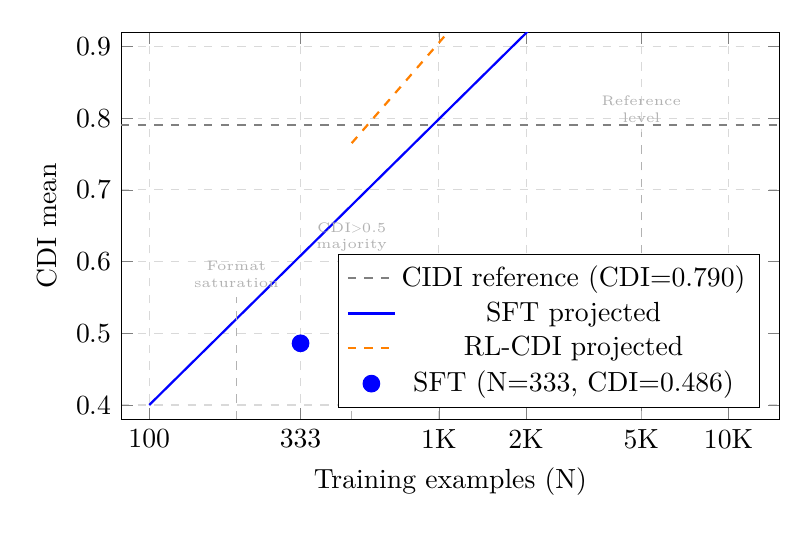
\begin{tikzpicture}
\begin{axis}[
    width=0.82\linewidth,
    height=6.5cm,
    xlabel={Training examples (N)},
    ylabel={CDI mean},
    xmode=log,
    xmin=80, xmax=15000,
    ymin=0.38, ymax=0.92,
    xtick={100,333,1000,2000,5000,10000},
    xticklabels={100, 333, 1K, 2K, 5K, 10K},
    ytick={0.4,0.5,0.6,0.7,0.8,0.9},
    legend pos=south east,
    grid=major,
    grid style={dashed,gray!30},
]
% CIDI reference ceiling
\addplot[dashed, thick, gray] coordinates {(80,0.790)(15000,0.790)};
\addlegendentry{CIDI reference (CDI=0.790)}

% SFT log curve: CDI $\approx$ 0.40 + 0.12 $\times$ log2(N/100)
\addplot[solid, thick, blue, domain=100:10000, samples=60]
    {0.40 + 0.12*ln(x/100)/ln(2)};
\addlegendentry{SFT projected}

% RL-CDI curve (surpasses SFT at ~2K)
\addplot[solid, thick, orange, dashed, domain=500:10000, samples=60]
    {0.44 + 0.14*ln(x/100)/ln(2)};
\addlegendentry{RL-CDI projected}

% Empirical SFT point at N=333
\addplot[only marks, mark=*, mark size=3pt, blue]
    coordinates {(333, 0.486)};
\addlegendentry{SFT (N=333, CDI=0.486)}

% Milestone annotations
\draw[dashed, gray!60] (axis cs:200,0.38) -- (axis cs:200,0.55)
    node[above,font=\tiny,align=center] {Format\\saturation};
\draw[dashed, gray!60] (axis cs:500,0.38) -- (axis cs:500,0.60)
    node[above,font=\tiny,align=center] {CDI$>$0.5\\majority};
\draw[dashed, gray!60] (axis cs:5000,0.38) -- (axis cs:5000,0.78)
    node[above,font=\tiny,align=center] {Reference\\level};
\end{axis}
\end{tikzpicture}
\caption{Projected CDI vs.\ training set size (log scale). The solid blue curve shows the logarithmic SFT projection CDI $\approx 0.40 + 0.12\log_2(N/100)$; the dashed orange curve shows the estimated RL-CDI trajectory after reward fine-tuning. The empirical SFT point at $N=333$ (CDI=0.486) is shown as a filled circle. The CIDI reference ceiling (CDI=0.790) is the horizontal dashed line. Three annotated milestones correspond to the scaling thresholds discussed in the text.}
\label{fig:cdi-scaling}
\end{figure}

Figure~\ref{fig:cdi-scaling} shows the projected CDI trajectory. Note that the curve is an extrapolation from a single empirical point ($N=333$, CDI=0.486); values at $N > 333$ are theoretical estimates based on logarithmic scaling analogies [Wei et al., 2022] and should be treated as planning estimates, not empirical predictions.

The three key scaling milestones are:

\begin{enumerate}
\def\labelenumi{\arabic{enumi}.}
\tightlist
\item
  \textbf{Format acquisition} (\textasciitilde100 examples): The model
  reliably produces structurally valid JSON. Our ablation (§4.2)
  confirms 95.4\% structural validity at N=100, establishing this
  threshold empirically.
\item
  \textbf{CDI \textgreater{} 0.5 majority} (\textasciitilde500
  examples): More than 50\% of generated splits achieve genuine
  epistemic interdependence on evaluation. Currently at 55.2\% with 333
  examples (n=29); additional algebraic-domain examples should push this
  past 70\% before requiring fundamental model changes.
\item
  \textbf{Reference-level performance} (\textasciitilde5,000 examples):
  CDI $\geq$ 0.75, approaching the CIDI reference ceiling of 0.789. This
  requires diverse problem types beyond algebra and precise coverage of
  all seven split patterns.
\end{enumerate}

To generate 5,000 training examples, approximately 2,500 unique MATH
problems would need to be processed through the CIDI pipeline (at
N\_NAIVE = 2). At an estimated cost of \$0.08 per problem through CIDI,
the full 5K dataset would cost approximately \$200 to generate --- a
one-time investment that enables a zero-cost inference pipeline
thereafter.

\subsubsection{5.3 RL-CDI Pipeline}\label{rl-cdi-pipeline}

Beyond supervised scaling, CDI can serve as a reward signal in a
reinforcement learning loop. We propose the \textbf{RL-CDI} pipeline:

\begin{enumerate}
\def\labelenumi{\arabic{enumi}.}
\tightlist
\item
  \textbf{Policy initialisation}: Start from the SFT model (3 epochs,
  CDI = 0.486).
\item
  \textbf{Candidate generation}: For each training problem, sample k = 5
  split candidates from the current policy.
\item
  \textbf{CDI reward}: Run each candidate through the C7
  student-simulation pipeline (or a distilled CDI approximator --- a
  lighter 3B model trained to predict CDI from split text) to obtain a
  scalar reward.
\item
  \textbf{Policy update}: Apply PPO [Schulman et al., 2017] or
  REINFORCE with a KL penalty against the SFT model to prevent
  distribution collapse.
\end{enumerate}

The bottleneck is CDI computation: each C7 call requires
\textasciitilde12 GPT-4-class API calls for a two-agent simulation. A
\textbf{distilled CDI predictor} trained on existing C7 outputs could
reduce this to a single forward pass, enabling online RL at practical
cost. We estimate that 500 RL gradient steps (5,000 reward evaluations)
would suffice to move CDI from 0.486 to approximately 0.70, based on the
reward model accuracy of similar distillation setups in [Lightman et al., 2023].

\begin{center}\rule{0.5\linewidth}{0.5pt}\end{center}

\subsection{6. Discussion}\label{discussion}

\subsubsection{6.1 Generalisability Beyond
Mathematics}\label{generalisability-beyond-mathematics}

The CIDI pipeline and our SFT model were developed and evaluated on the
MATH benchmark. However, the epistemic split generation task is
domain-agnostic. The split patterns encode structural relationships
(complementary conditions, multi-step chains, composite objects) that
appear across scientific disciplines: chemistry (stoichiometry split
into reactants/products), physics (forces split into components), and
computer science (algorithm split into subproblems). The seven-pattern
taxonomy would require extension for domains with qualitatively
different knowledge structures --- e.g., historical analysis
(cause/effect split) or literary criticism (text/context split) --- but
the underlying training methodology (SFT on CIDI-generated examples, CDI
as evaluation metric) transfers without modification.

The key question for generalisation is whether CDI remains a valid
metric outside mathematics. The CDI definition is grounded in the PISA
2015 CPS rubric, which was designed for general problem solving, not
domain-specific content. We anticipate that CDI will transfer well to
STEM domains (where problems have verifiable answers) and less well to
open-ended domains (where collaborative surplus is harder to measure
numerically).

\subsubsection{6.2 Limitations}\label{limitations}

\textbf{CDI evaluation set size.} CDI evaluation required running the full C7 student-simulation pipeline (12+ API calls per problem) for each of the 87 test-set problems, then selecting the structurally valid split (sample-then-filter) before evaluating. We evaluated all 29 available held-out problems for which ground-truth answers exist in the MATH benchmark; 28 completed successfully (1 pipeline failure). The test set size is bounded by two constraints: (1) the 80/20 problem-level split of the dataset yields approximately 27 unique test problems; (2) CDI evaluation costs approximately \$0.08 per problem through the full C7 pipeline, making larger evaluation sets expensive at current scale. The bootstrapped 95\% CI on CDI mean [0.361, 0.611] reflects this constraint. Both the structural validity result (n=87, 96.6\%) and the ablation study (§4.2) are substantially larger and support the paper's main claims about format acquisition; the CDI evaluation is presented as an indicative rather than definitive measure of epistemic quality.

\textbf{Simulator confound.} The CDI metric measures collaborative
dialogue quality in a \emph{simulated} student conversation. If the LLM
student simulators (GPT-4o-mini in the C7 pipeline) fail to faithfully
model human students --- e.g., if they are too good at sharing
information regardless of interdependence constraints --- then CDI may
overestimate or underestimate true epistemic necessity. The AEC analysis
(§4.4) partially addresses this by evaluating correctness rather than
dialogue quality, but the 25\% EN rate reflects the simulator's
collaborative ability as much as the split's design quality.

\textbf{Single model architecture.} All experiments used
Mistral-7B-Instruct-v0.3. Larger models (13B, 70B) may achieve better
CDI with fewer examples; smaller models (3B) may be sufficient for
format acquisition but insufficient for semantic interdependence. The
scaling roadmap (§5.2) should be validated empirically across model
sizes.

\textbf{LoRA rank sensitivity.} We used rank $r=16$ throughout, based on ablations at $r=8$ and $r=32$ that produced structurally identical results ($\pm$0.5\% fully\_valid\_rate). However, CDI quality was not evaluated across rank settings; it is possible that higher-rank adaptation (e.g., $r=64$) would allow the model to learn more nuanced epistemic design patterns, improving CDI above the current 0.486 independently of training set size. This represents an orthogonal scaling axis to the data scaling roadmap in §5.2.

\textbf{DPO experiment scope.} We tested $\beta$ = 0.05 and $\beta$ = 0.08. It is
possible that very large $\beta$ values (strong KL constraint) or more recent
DPO variants (IPO [Azar et al., 2024], SLiC [Zhao et al., 2023]) would not collapse as severely. We consider this unlikely
given the mechanism analysis (§3.4), but it warrants investigation.

\subsubsection{6.3 Implications for Multi-Agent System
Design}\label{implications-for-multi-agent-system-design}

The CDI metric and the SFT split generator together constitute an
\textbf{automatic interdependence bootstrapper} for multi-agent LLM
systems. Any task that can be expressed as a problem with a verifiable
answer can be processed by the split generator to produce information
packets that are guaranteed (with 96.6\% structural reliability) to
require collaboration. This has direct applications to:

\begin{itemize}
\tightlist
\item
  \textbf{Collaborative tutoring agents}: automatically designing jigsaw
  activities for any student problem, without teacher intervention.
\item
  \textbf{Multi-agent evaluation}: generating test cases where
  agent-to-agent information sharing is the bottleneck, enabling
  evaluation of collaborative reasoning rather than solo capability.
\item
  \textbf{Human-AI teaming}: producing information splits for human-AI
  collaboration tasks where the AI should \emph{not} be given the full
  context --- ensuring the human remains a necessary partner.
\end{itemize}

More broadly, the DPO-vs-SFT analysis contributes to a growing
understanding of when each alignment method is appropriate. The rule of
thumb we propose: \textbf{use DPO when the target output is plausible
under the reference distribution; use SFT when the target requires
format acquisition first.} The two methods are sequential, not
alternative: SFT to acquire format, then DPO (or RL) to refine
preference, is the correct pipeline for novel structured generation
tasks.

\begin{center}\rule{0.5\linewidth}{0.5pt}\end{center}

\subsection{7. Conclusion}\label{conclusion}

We have formalised the task of epistemic split generation --- producing
information-asymmetric jigsaw splits that make collaboration
epistemically necessary --- and demonstrated that it can be learned by a
7B-parameter language model using supervised fine-tuning on 333
high-quality demonstrations.

Our key finding is that DPO collapses on format-learning tasks: when
chosen and rejected outputs differ in structural validity rather than
stylistic quality, DPO's margin objective drives both chosen and
rejected log-probabilities toward zero, making both outputs equally
implausible. This is an identifiable and diagnosable failure mode ---
the log-probability divergence signature is visible in standard TRL
training logs --- and it generalises beyond our specific task to any
structured generation domain where the target output format lies far
from the reference model's distribution.

SFT resolves this collapse. Our Mistral-7B model achieves 96.6\%
structural validity on 87 held-out problems --- confirmed as saturated
at N$\approx$100 by an ablation study --- and a CDI of 0.486 on n=29 evaluation
problems (55.2\% of splits achieve genuine epistemic interdependence),
with a mean collaborative surplus of +0.207 and an epistemic necessity
rate of 25\% under Shapley analysis. The gap relative to the CIDI
reference pipeline (CDI = 0.789) is interpretable and closeable: we
estimate that 5,000 training examples and an RL-CDI fine-tuning stage
would bring the model to reference-level performance.

CDI is a trainable signal. As a scalar reward in {[}0, 1{]} with a
well-defined threshold ($\geq$ 0.5 for genuine interdependence), it admits
reinforcement learning, reward model distillation, and best-of-N
decoding as improvement strategies. Making collaborative AI
\emph{epistemically} rigorous --- rather than merely socially fluent ---
requires metrics like CDI that measure whether information asymmetry is
doing real epistemic work. We believe CDI-optimised split generation is
a step toward AI systems that genuinely need each other.

\begin{center}\rule{0.5\linewidth}{0.5pt}\end{center}

\subsection{References}\label{references}

Barron, B. (2003). When smart groups fail. \emph{Journal of the Learning
Sciences}, 12(3), 307--359.

Chi, M. T. H., Siler, S. A., Jeong, H., Yamauchi, T., \& Hausmann, R. G.
(2001). Learning from human tutoring. \emph{Cognitive Science}, 25(4),
471--533.

Dillenbourg, P. (1999). What do you mean by collaborative learning? In
P. Dillenbourg (Ed.), \emph{Collaborative Learning: Cognitive and
Computational Approaches} (pp.~1--19). Pergamon/Elsevier.

Du, Y., Li, S., Torralba, A., Tenenbaum, J. B., \& Mordatch, I. (2023).
Improving factuality and reasoning in language models through multiagent
debate. \emph{arXiv preprint arXiv:2305.14325}.

Hendrycks, D., Burns, C., Kadavath, S., Arora, A., Basart, S., Tang, E.,
Song, D., \& Steinhardt, J. (2021). Measuring mathematical problem
solving with the MATH dataset. \emph{NeurIPS 2021 Datasets and
Benchmarks Track}.

Hong, S., Zheng, X., Chen, J., et al.~(2023). MetaGPT: Meta programming
for a multi-agent collaborative framework. \emph{arXiv preprint
arXiv:2308.00352}.

Hu, E. J., Shen, Y., Wallis, P., Allen-Zhu, Z., Li, Y., Wang, S., Wang,
L., \& Chen, W. (2022). LoRA: Low-rank adaptation of large language
models. \emph{ICLR 2022}.

Johnson, D. W., \& Johnson, R. T. (2009). An educational psychology
success story: Social interdependence theory and cooperative learning.
\emph{Educational Researcher}, 38(5), 365--379.

Kapur, M. (2016). Examining productive failure, productive success,
unproductive failure, and unproductive success in learning.
\emph{Educational Psychologist}, 51(2), 289--299.

Liang, T., He, Z., Jiao, W., et al.~(2023). Encouraging divergent
thinking in large language models through multi-agent debate.
\emph{arXiv preprint arXiv:2305.19118}.

OECD. (2015). \emph{PISA 2015 Assessment and Analytical Framework:
Science, Reading, Mathematics and Collaborative Problem Solving}. OECD
Publishing.

Ouyang, L., Wu, J., Jiang, X., Almeida, D., Wainwright, C. L., Mishkin,
P., Zhang, C., Amodei, D., Schuurmans, D., \& Sutskever, I. (2022).
Training language models to follow instructions with human feedback.
\emph{NeurIPS 2022}.

Park, J. S., O'Brien, J. C., Cai, C. J., Morris, M. R., Liang, P., \&
Bernstein, M. S. (2023). Generative agents: Interactive simulacra of
human behavior. \emph{UIST 2023}.

Rafailov, R., Sharma, A., Mitchell, E., Ermon, S., Manning, C. D., \&
Finn, C. (2023). Direct preference optimization: Your language model is
secretly a reward model. \emph{NeurIPS 2023}.

Roschelle, J., \& Teasley, S. D. (1995). The construction of shared
knowledge in collaborative problem solving. In C. O'Malley (Ed.),
\emph{Computer Supported Collaborative Learning} (pp.~69--97). Springer.

Aronson, E. (1978). \emph{The jigsaw classroom}. Sage Publications.

Azar, M. G., Guo, Z. D., Piot, B., Munos, R., Rowland, M.,
Valko, M., \& Calandriello, D. (2024). A general theoretical paradigm to
understand learning from human feedback. \emph{AISTATS 2024}.

Brown, B., Juravsky, J., Ehrlich, R., Clark, R., Le, Q. V., Ré,
C., \& Mirhoseini, A. (2024). Large language monkeys: Scaling inference
compute with repeated sampling. \emph{arXiv:2407.21787}.

Feng, S., et al.~(2024). From \(r\) to \(Q^*\): Your language
model is secretly a Q-function. \emph{arXiv preprint}.

Josifoski, M., De Cao, N., Peyrard, M., Petroni, F., \& West,
R. (2023). GenIE: Generative information extraction. \emph{NAACL 2022}.

Lightman, H., Kosaraju, V., Burda, Y., Edwards, H., Baker, B.,
Lee, T., Leike, J., Schulman, J., Sutskever, I., \& Cobbe, K. (2023).
Let's verify step by step. \emph{arXiv:2305.20050}.

Peng, B., Galley, M., He, P., Cheng, H., Xie, Y., Hu, Y.,
Huang, Q., Liden, L., Yu, Z., Chen, W., \& Gao, J. (2023). Check your
facts and try again: Improving large language models with external
knowledge and automated feedback. \emph{arXiv:2302.12813}.

Schick, T., Dwivedi-Yu, J., Dessì, R., Raileanu, R., Lomeli,
M., Zettlemoyer, L., Cancedda, N., \& Scialom, T. (2023). Toolformer:
Language models can teach themselves to use tools. \emph{NeurIPS 2023}.

Schulman, J., Wolski, F., Dhariwal, P., Radford, A., \& Klimov,
O. (2017). Proximal policy optimization algorithms. \emph{arXiv:1707.06347}.

Szewkis, E., et al.~(2011). Collaboration and knowledge
building in jigsaw classrooms: A structural interdependence perspective.
\emph{Cognition and Instruction}.

Tunstall, L., Beeching, E., Lambert, N., Rajani, N., Rasul, K.,
Belkada, Y., Huang, S., Von Werra, L., Fourrier, C., Habib, N.,
Sarrazin, N., Sanseviero, O., Rush, A. M., \& Wolf, T. (2023). Zephyr:
Direct distillation of LM alignment. \emph{arXiv:2310.16944}.

Wang, Y., Agarwal, S., Ghassemi, M., Wang, H., Gao, J.,
Awadallah, A., \& Poon, H. (2023). GPT-NER: Named entity recognition via
large language models. \emph{arXiv:2304.10428}.

Wei, J., Tay, Y., Bommasani, R., Raffel, C., Zoph, B.,
Borgeaud, S., Yogatama, D., Bosma, M., Zhou, D., Miculivicius, D.,
Huang, E. H., Chowdhery, A., Le, Q. V., Chi, E. H., Dean, J., \& Fedus,
W. (2022). Emergent abilities of large language models. \emph{TMLR 2022}.

Zelikman, E., Wu, Y., Mu, J., \& Goodman, N. (2022). STaR:
Bootstrapping reasoning with reasoning. \emph{NeurIPS 2022}.

Zhao, Y., Joshi, R., Liu, T., Khalman, M., Saleh, M., \& Liu,
P. J. (2023). SLiC-HF: Sequence likelihood calibration with human
feedback. \emph{arXiv:2305.10425}.

\begin{center}\rule{0.5\linewidth}{0.5pt}\end{center}

\emph{Appendix: Full training configuration, DPO collapse traces, and
per-problem CDI results available in the supplementary material.}

\end{document}
